\documentclass[a4paper,11pt]{book}


\usepackage[T1]{fontenc}

% \usepackage{mathpazo}
\linespread{1.05}
\usepackage{palatino}
% \usepackage{carolmin}

\usepackage{a4wide}
\usepackage{booktabs}

\usepackage{xspace}

\usepackage{graphics}
\usepackage{epsfig}

\usepackage{url}
\usepackage[pdftex, hyperindex=true, colorlinks=true, unicode, implicit=true,
linkcolor=blue, anchorcolor=magenta, citecolor=blue, urlcolor=blue]{hyperref}

\usepackage{amsmath}
\usepackage{amssymb}
\usepackage[squaren]{SIunits}


\usepackage{longtable}

\usepackage[dvipsnames,usenames]{color}
\usepackage{xcolor}

\usepackage{listings}

\usepackage{makeidx}

\usepackage[lofdepth,lotdepth]{subfig}
\usepackage{tikz}
\usetikzlibrary{decorations}


% \usepackage{fancybox}
% \usepackage{alltt}
% \usepackage{array}
% \usepackage{verbatim}
% \usepackage{ae}
% \usepackage{aecompl}
% \usepackage[cm]{aeguill}
% \usepackage{times}
% \usepackage{bookman}


\definecolor{RED}{rgb}{1,0,0}
\definecolor{cppbg}{HTML}{EBF2F2}
\definecolor{shellbg}{HTML}{F5EDE4}
\definecolor{commentcolor}{HTML}{101280}

\lstdefinestyle{C++}{
  language=C++, % the language of the code
  basicstyle=\small\ttfamily, % Without beramono, we'd get cmtt, the teletype font.
  commentstyle=\color{commentcolor}\itshape,
  keywordstyle=\color{DarkOrchid}\bfseries,
  % fontadjust,
  % numbers=left, % where to put the line-numbers
  % numberstyle=\tiny, % the size of the fonts that are used for the line-numbers
  % stepnumber=2, % the step between two  line-numbers.  If it's 1, each line will
  % be numbered
  % numbersep=5pt, % how far the line-numbers are from the code
  % showspaces=false, % show spaces adding particular underscores
  showstringspaces=false, % underline spaces within strings
  % showtabs=false, % show tabs within strings adding particular underscores
  % frame=llines, % adds a frame around the code
  % frame=tb,
  tabsize=2, % sets default tabsize to 2 spaces
  captionpos=b, % sets the caption-position to bottom
  breaklines=true, % sets automatic line breaking
  breakatwhitespace=false,   % sets if  automatic breaks  should only  happen at
  % whitespace
  % title=\lstname, % show the filename of files included with \lstinputlisting;
  % also try caption instead of title
  % escapeinside={\%*}{*)}, % if you want to add a comment within your code
  xleftmargin=1cm,
  xrightmargin=1cm,
  mathescape=true,
  escapechar=\%,
  morekeywords={Real, UInt, Int},
  columns=flexible,
  keepspaces=true,
  backgroundcolor=\color{cppbg}
}

\lstdefinestyle{shell}{
  language=bash, % the language of the code
  basicstyle=\scriptsize\ttfamily, % Without beramono, we'd get cmtt, the teletype font.
  showstringspaces=false, % underline spaces within strings
  tabsize=2, % sets default tabsize to 2 spaces
  captionpos=b, % sets the caption-position to bottom
  breaklines=true, % sets automatic line breaking
  breakatwhitespace=false,
  xleftmargin=1cm,
  xrightmargin=1cm,
  escapechar=\%,
  morekeywords={mkdir, make, ccmake, cmake},
  columns=flexible,
  keepspaces=true,
  backgroundcolor=\color{shellbg}
}

\lstnewenvironment{cpp}{\lstset{style=C++}}{}
\lstnewenvironment{command}{\lstset{style=shell}}{}
\makeatletter
\def\lst@outputspace{{\ifx\lst@bkgcolor\empty\color{white}\else\lst@bkgcolor\fi\lst@visiblespace}}
\makeatother

\renewcommand{\labelitemi}{$\mathbf{\circ}$}

\sloppy

\newcommand{\version}{0.1}
\newcommand{\akantu}{{\texttt{\textbf{Akantu}}}\xspace}

\newcommand{\code}[1]{\texttt{#1}}
\newcommand{\note}[1]{\textbf{Note: }\textit{#1}}
\newcommand{\todo}[1]{~({\small\color{red}\textbf{TODO: }\textbf{#1}})}

\renewcommand{\vec}[1]{\ensuremath{\boldsymbol{#1}}}
\newcommand{\mat}[1]{\ensuremath{\boldsymbol{#1}}}
\newcommand{\st}[1]{{\mathrm{#1}}}

\newcommand{\eg}{\emph{e.g.}\xspace}
\newcommand{\ie}{\emph{i.e.}\xspace}

\bibliographystyle{plain}

\title{\textbf{\Huge \akantu}\\
  \vspace{0.5cm}
  \textbf{\huge User's Guide}\\
  \vspace{1cm}
  {\small \today{} --- Version \version}
}

\date{}

\makeindex

\begin{document}

\maketitle

\tableofcontents

\chapter{Introduction}

% \section{Data structures\label{chap:data-structure}}

% \subsection{Vectors\label{sec:vectors}}

% The Vector class is a template class  that can store scalar types as Real, UInt,
% Int  or bool.   A Vector  instance is  defined  by its  size and  its number  of
% component.  It also  has an  identifier and  some extra  internal  variables for
% memory handling purpose.

% \begin{itemize}
% \item The size is the number of tupels stored in the Vector.
% \item The number of component is the number of values stored for each tuple.
% \end{itemize}

% \begin{figure}[!htb]
%   \centering
%   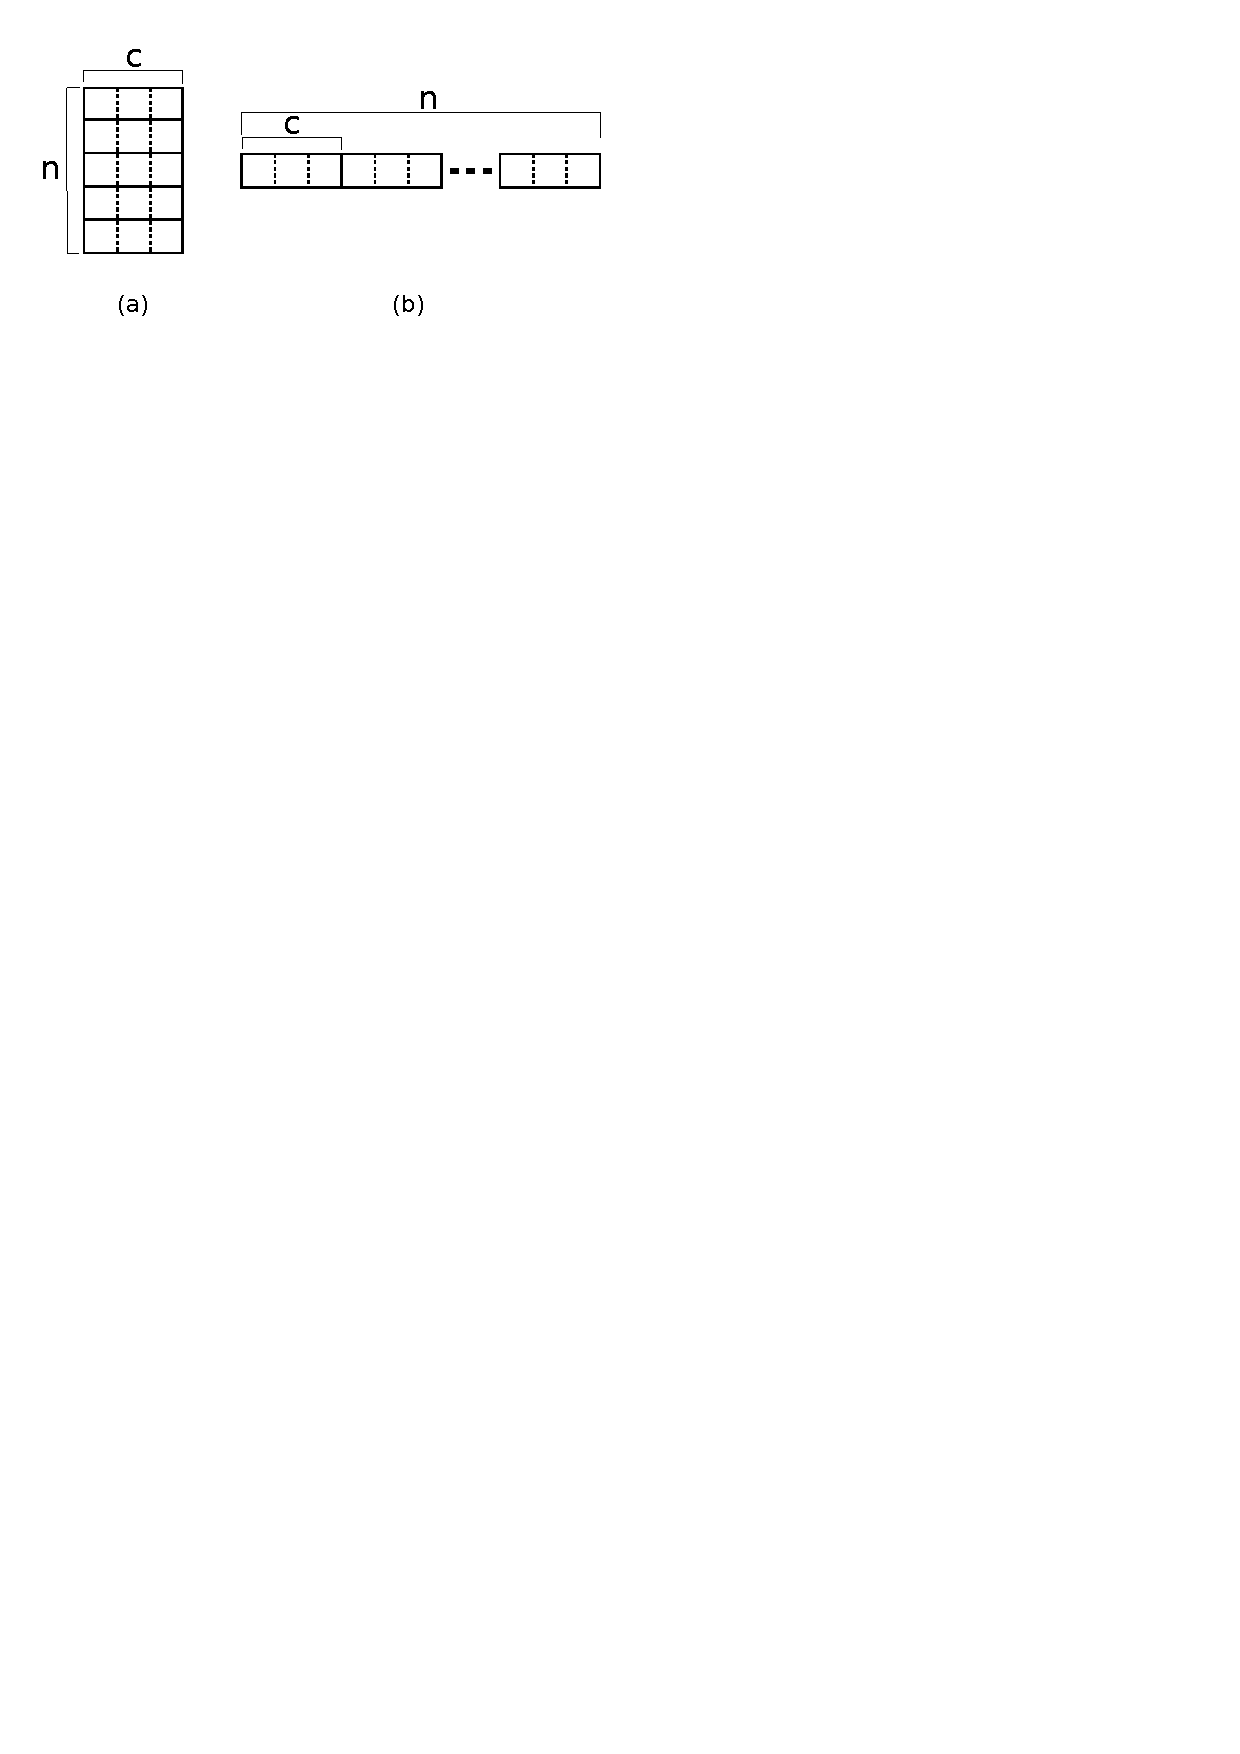
\includegraphics{figures/vectors}
%   \caption{View of  a Vector of size  n and c compenents,  (a) representation of
%     the vector, (b) representation of the storage of the same Vector.}
%   \label{fig:vectors}
% \end{figure}

% All the  data are linerarized  in memory in  an array called values.  This class
% member is public.  So for a Vector  of size $n$ and $c$ component, to access the
% $j^{th}$  component of  th  $i^{th}$ tuple,  you have  to  get $values[i  * c  +
% j]$. You  can also  access to this  value with  accessor \code{at(i, j)}  or the
% constant accessor \code{get(i, j)}.

% If  you want to  store a  matrix on  each tuple  you have  to linearize  it. For
% exemple if you want to store a m * k matrix on each tuple you must specify c = m
% * k.  To access a particular value  in a matrix of  a tuple you will  have to do
% something like $values[ i * m * k + j_i * m + j_j]$.

% \subsubsection{Vector storage convention within FE object\label{sec:FE-convention}}

% The point of  this section is to describe the convention  of storage for vectors
% intented  to be  passed to  {\bf  FE} object  methods.  Indeed  a convention  of
% necessary  since gradient  operators or  integrtaion loops  will use  vectors as
% input and ouput.   Such vectors will be ordered with  a specific convention that
% we intend to describe now.

% For  vector objects,  the  size of  the vector  is  always the  number of  nodes
% associated.  The number  of components  is related  to the  order of  the tensor
% considered. For a scalar  field it is 1, for a vectorial  field, the size of the
% vector is the number of components. For a $m\times n$ matrix field the number of
% components is $m\times n$.

% One common operation  is the manipulation of continuum  fields at the quadrature
% point  positions.   Here  the  size   of  the  vector  is   $mn\_element  \times
% nb\_quad\_points$  and  the  number  of  components is  related  to  the  stored
% object.  For instance the  method \verb$interpolateOnQuadraturePoints()$  take a
% nodal field  stored in a  vector($n\_nodes$,$dim$) and return  a vector($n\_elem
% \times n\_quads$,$dim$).

% Basic gradient operations, like method \verb$gradientOnQuadraturePoints()$, will
% take  as input a  vector($n\_nodes$,$dim$) and  return a  vector($n\_elem \times
% n\_quads$,$dim \times spatial\_dimension$) where spatial dimension is the number
% of dimension in which the domain is embedded.

% In  the  same  way   the  integration  routines  expect  vector($n\_elem  \times
% n\_quads$,$dim$)  and  will  return vector($n\_elem$,$dim$).   For  non-Gaussian
% integrations, the input  by be direction a nodal field.   (At present time, only
% gaussian integrators are implemented within akantu).

% Last but  not the least  is the vectorial  assembly process for which  accept as
% input vector($n\_elem \times n\_quads \times n\_nodes\_per\_element$,$dim$)
% and will return a vector($n\_nodes$,$dim$) nodal object.\\

% {\bf The general convention is that  the number of component shall always be the
%   size of  the object manipulated  at the lowest  level.  The object could  be a
%   per-element, of  per quadrature point  or even per  node basis this  will also
%   apply    as   shown    below.   The    figures    \ref{fig:vector-chain}   and
%   \ref{fig:interpolate-storage} shows the  pattern of the vectors is  the case a
%   interpolation on quadrature points.}

% \begin{figure}
%   \begin{equation}
%     \left(
%       \begin{array}{c}
%         N_1 \\
%         \vdots \\
%         N_I
%         \left\{
%           \begin{array}{c}
%             a_1 \\
%             \vdots \\
%             a_{dim} \\
%           \end{array}
%         \right. \\
%         \vdots \\
%         N_{nb\_nodes}
%       \end{array}
%     \right)
%     \begin{array}{c}
%       \Longrightarrow \\
%       interpolate\\
%       On\\
%       Quadrature\\
%       Points\\
%     \end{array}
%     \left(
%       \begin{array}{c}
%         E_1 \\
%         \vdots \\
%         E_e
%         \left\{
%           \begin{array}{c}
%             q_1 \\
%             \vdots \\
%             \left.
%               \begin{array}{c}
%                 a_1 \\
%                 \vdots \\
%                 a_{dim}
%               \end{array}
%             \right\} q_i \\
%             \vdots \\
%             q_p \\
%           \end{array}
%         \right.  \\
%         \vdots \\
%         E_{nb\_elements}
%       \end{array}
%     \right)
%   \end{equation}
%   \caption{\label{fig:vector-chain}Pattern   of   vectors   manipulated   during
%     interpolation on  quadrature points.  Symbols  N (resp. E, q)  denotes nodes
%     (resp. elements, quadrature points).}
% \end{figure}

% \begin{figure}[!htb]
%   \centering
%   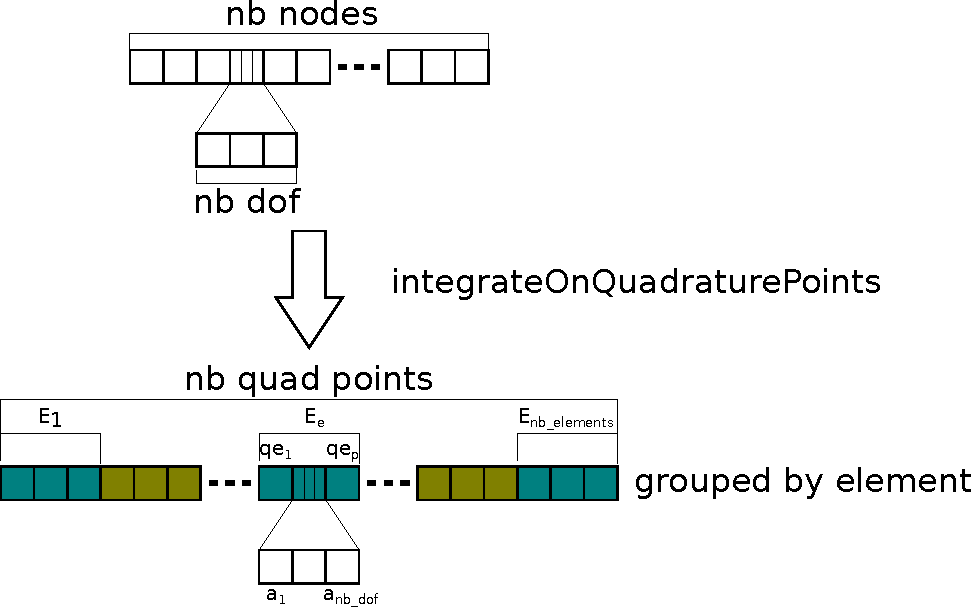
\includegraphics[width=\textwidth]{figures/interpolate}
%   \caption{Input and output  vector of interpolateOnQuadraturePoints. The output
%     Vector has nb\_quadrature\_points tuples,  the quadrature points are grouped
%     by elements (p is the number of quadrature points per element).}
%   \label{fig:interpolate-storage}
% \end{figure}

\chapter{Planning}

\begin{description}
\item[03/12/12] Cyprien: Explicit time integration scheme
\item[03/29/12] Aurelia: Boundary conditions
\item[04/13/12] Leonardo: Existing constitutive laws
\item[04/20/12] Mohadeseh: Adding a constitutive law
\item[04/27/12] Peter: Adding an element
\item[05/04/12] Till: Structural mechanics model
\item[05/11/12] Guillaume: Heat transfer model
\item[05/18/12] Marco: Cohesive elements
\item[05/25/12] Alejandro: Contact detection
\item[06/01/12] David: Contact resolution
\end{description}

\begin{figure}[!htb]
  \centering
  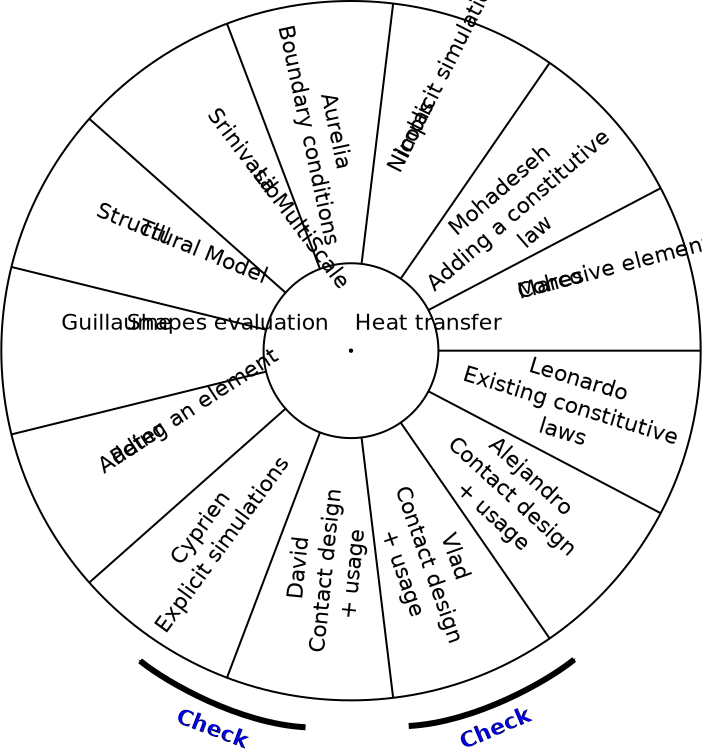
\includegraphics[width=\linewidth]{figures/doc_wheel}
  \caption{Documentation wheel\label{fig:doc_wheel}}
\end{figure}

\chapter{How to use Akantu}
\section{Getting started}
\subsection{Downloading the code}
SVN URL to get \akantu :
\begin{command}
  > svn co svn+ssh://username@intranet-lsms.epfl.ch/space/repositories/SimulPack/akantu/trunk akantu
\end{command}

\subsection{Compiling Akantu}
\begin{command}
  > mkdir build
  > cd build
  > ccmake <path to akantu sources>
\end{command}

Set the options that you need

\begin{command}
  > make
  > make install
\end{command}

\subsection{Creating and loading a mesh\label{sect:common:mesh}}

\begin{cpp}
  UInt spatial_dimension = 2;

  Mesh mesh(spatial_dimension);

  MeshIOMSH mesh_io;
  mesh_io.read("square.msh", mesh);
\end{cpp}

\section{Solid Mechanics Model\index{SolidMechanicsModel}}

The  solid mechanics  model is  a  specific implementation  of the  \code{Model}
interface  dedicated  to  handle  the   equations  of  motion  or  equations  of
equilibrium. The  model is  created for a  given mesh.   It will create  its own
\code{FEM}  object  to  compute  the interpolation,  gradient,  integration  and
assembly operations.  A \code{SolidMechanicsModel}  object can simply be created
like this:
\begin{cpp}
  SolidMechanicsModel model(mesh, spatial_dimension);
\end{cpp}
where \code{mesh}  is the  mesh for which  the equations  are to be  solved, and
\code{spatial\_dimension}  is  the  dimensionality   of  the  problem.   If  the
\code{spatial\_dimension} is  omitted, the  problem is assumed  to have  the same
dimensionality as the one specified by the mesh.

This model contains at least the the following six \code{Vectors}:
\begin{description}
\item[boundary]  contains a  \code{boolean}  value for  each  degree of  freedom
  specifying  whether  that degree  is  blocked  or  not. A  Dirichlet  boundary
  condition can be prescribed by setting the \textbf{boundary} value of a degree
  of freedom to  \code{true}.  A Neumann boundary condition  can only be applied
  if the  \textbf{boundary} value of a  degree of freedom is  \code{false}. If a
  degree  of freedom  has a  \textbf{boundary} value  that is  \code{false}, the
  \textbf{displacement},     \textbf{velocity},     \textbf{acceleration}    and
  \textbf{residual} are computed by the solve algorithm when relevant, otherwise
  these  vectors  contain   the  imposed  value  (zero  by   default  after  the
  initialization).
\item[displacement] contains the displacements of all degrees of freedom. It can
  be either  a computed displacement for  free degrees of freedom  or an imposed
  displacement in case of blocked ones ($\vec{u}$ in the following).
\item[velocity]  contains  the  velocities   of  all  degrees  of  freedom.   As
  \textbf{displacement}, it contains computed or imposed velocities depending on
  the nature of the degrees of freedom ($\vec{\dot{u}}$ in the following).
\item[acceleration]  contains the accelerations  of all  degrees of  freedom. As
  \textbf{displacement}, it contains computed or imposed accelerations depending
  on the nature of the degrees of freedom ($\vec{\ddot{u}}$ in the following).
\item[force]   contains    the   external   forces   applied    on   the   nodes
  ($\vec{f_{\st{ext}}}$ in the following).
\item[residual] contains the difference between external and internal forces. On
  blocked degrees of freedom,  \textbf{residual} contains the support reactions.
  ($\vec{r}$  in the  following).  It  should be  mentioned that  at equilibrium
  \textbf{residual} should be zero on free degrees of freedom.
\end{description}

Some examples for to help to understand  how to use this model will be presented
in the next sections.

\subsection{Model setup}

\subsubsection{Setting   initial  conditions  \label{sect:smm:initial_condition}}

For  a unique  solution of  the equations  of motion  initial  displacements and
velocities at time $t=0$ at all degrees of freedom must be specified.

\begin{eqnarray}
  \vec{u(t=0)} = \vec{u}_{0}\\
  \vec{\dot u(t=0)} = \vec{v}_{0}
\end{eqnarray}
The solid mechanics model can be initialized as follows:
\begin{cpp}
  model.initFull("material.dat")
\end{cpp}
This function  initializes the internal vectors  and sets them  to zero. Initial
displacements and  velocities that are  not equal to  zero can be  prescribed by
running a  loop over the total  number of nodes. Here,  the initial displacement
and in x-direction  and the initial velocity in y-direction at  all nodes is set
to $0.1$ and $1$ respectively.
\begin{cpp}
  Vector<Real> & disp = model.getDisplacement();
  Vector<Real> & velo = model.getVelocity();
  for (UInt i = 0; i < nb_nodes; ++i) {
    disp(i, 0) = 0.1;
    velo(i, 1) = 1.;
  }
\end{cpp}
\subsubsection{Setting boundary conditions\label{sect:smm:boundary}}
This section explains how to  impose Dirichlet or Neumann boundary conditions. A
Dirichlet boundary condition specifies the values that the displacement needs to
take    at    the    boundary     ($\Gamma_u$)    of    the    problem    domain
(Fig.~\ref{fig:smm:boundaries}):
\begin{equation}
  \vec{u} = \vec{\bar u} \quad \forall \vec{x}\in \Gamma_{u}
\end{equation}
A  Neumann boundary  condition specifies  the values  that the  gradient  of the
solution  needs to  take  at the  boundary  ($\Gamma_t$) of  the problem  domain
(Fig.~\ref{fig:smm:boundaries}):
\begin{equation}
  \vec{t} = \mat{\sigma} \vec{n} = \vec{\bar t} \quad \forall \vec{x}\in \Gamma_{t}
\end{equation}
\begin{figure}[!htb]
  \centering
  \includegraphics[scale=0.6]{figures/boundary}
  \caption{Problem boundary in two dimensions.\label{fig:smm:boundaries}}
\end{figure}

Figure~\ref{fig:smm:dirichlet_bc} shows a beam with  a fixed support on the left
side. On the right end of the beam  a load is applied. At the fixed support, the
displacement has a  given value. For this example, the  displacement in both the
x-  and y-direction  is set  to  zero. Implementing  this displacement  boundary
condition is  similar to the  implementation of initial  displacement conditions
described above. However,  in order to impose a  displacement boundary condition
for all time steps, the corresponding  nodes need to be marked as boundary nodes
as shown in the following code:
\begin{cpp}
  Vector<bool> & boun = model.getBoundary();

  const Vector<Real> & pos = mesh.getNodes();

  UInt nb_nodes = mesh.getNbNodes();
  Real epsilon = Math::getTolerance();
  /* this  tolerance is  by default equal  to the  machine precision but  can be changed by using %\code{Math::setTolerance(value)}% */

  for (UInt i = 0; i < nb_nodes; ++i) {
    if(std::abs(pos(i, 0)) < epsilon) {
      boun(i, 0) = true;  //block displacement in x-direction
      boun(i, 1) = true;  //block displacement in y-direction

      disp(i, 0) = 0.;   //fixed displacement in x-direction
      disp(i, 1) = 0.;   //fixed displacement in y-direction
    }
  }
\end{cpp}
\begin{figure}[!htb]
  \centering
  \includegraphics[scale=0.4]{figures/dirichlet}
  \caption{Beam with fixed support.\label{fig:smm:dirichlet_bc}}
\end{figure}

If the Neumann boundary condition consists of a single load that is acting on one
node, the load can simply be prescribed in the force vector:
\begin{cpp}
  Vector<Real> & force = model.getForce();
  // force acting on node n:
  force(n, 0) = 10.; // x-direction
  force(n, 1) = 0.; // y-direction
\end{cpp}

In  the  case  of  a  surface   load  the  consistent  nodal  force  has  to  be
computed.  Therefore,  a  new  class  \code{MySurfaceLoadFunctor}  needs  to  be
created,  which inherits  from  the class  \code{SolidMechanicsModel}. The  call
operator of  this class needs to  be overloaded and the  following parameters in
the call operator need to be defined:
\begin{itemize}
\item The position where the load is applied.
\item The type of load (traction or stress).
\item The normal vector at the point of the surface.
\item The surface\_id of the surface where the load is applied.
\end{itemize}
\begin{cpp}
  Real bar_length = 10.;

  class MySurfaceLoadFunctor : public SolidMechanicsModel::SurfaceLoadFunctor {
    public:
    // if a traction vector is provided:
    void operator()(const types::Vector<Real> & position,
    types::Vector<Real> & traction,
    const types::Vector<Real> & normal,
    Surface surface_id) {
      Real epsilon = Math::getTolerance();
      if(std::abs(position(0) - bar_length) < epsilon) {
        force(0) = 10e9;
      }
    }

    // if a stress tensor is provided:
    void operator() (const types::Vector<Real> & position,
    types::Matrix & stress,
    const types::Vector<Real> & normal,
    Surface surface_id) {
      Real epsilon = Math::getTolerance();
      if(std::abs(position(0) - bar_length) < epsilon) {
        stress(0,0) = 10e9;
        stress(1,1) = 10e9;
      }
    }
  };
\end{cpp}

In order to apply the  load that has been defined in \code{MySurfaceLoadFunctor}
on a  corresponding surface, this  surface needs to  be created first.  This can
either be done in a mesh generator like Gmsh or directly in \akantu by using the
function \code{MeshUtils::buildFacets(mesh)}. Once the surface has been created,
a  FEM  object  containing  the  surface  elements  of  the  mesh  needs  to  be
generated. In the  next step, the shape functions, the  derivatives of the shape
functions   and    Jacobians   for   the    surface   elements   need    to   be
computed.  Subsequently, the  normals on  the quadrature  points of  the surface
elements  are  calculated  and  an instance  of  \code{MySurfaceLoadFunctor}  is
created. In the  last step, the load at the Gauss  quadrature points is computed
by using the function \code{computeForcesFromFunction}:
\begin{cpp}
  MeshUtils::buildFacets(mesh);

  FEM & fem_boundary = model.getFEMBoundary();
  fem_boundary.initShapeFunctions();
  fem_boundary.computeNormalsOnControlPoints();

  MySurfaceLoadFunctor boundary_force;
  model.computeForcesFromFunction(boundary_force, _bft_force);
\end{cpp}
\begin{itemize}
\item\code{model.getFEMBoundary()}  creates  a  FEM  object  that  contains  the
  surface elements of the mesh.
\item\code{fem\_boundary.initShapeFunctions()}  computes  the  shape  functions,
  their derivatives and the jacobians.
\item\code{fem\_boundary.computeNormalsOnControlPoints()}  computes  the normals
  at the quadrature points of the surface elements.
\item\code{model.computeForcesFromFunction(boundary\_force,\_bft\_force)}
  computes  the   forces  from   the  call  operator   defined  in   the  object
  \code{boundary\_force}.       The      second      parameter      of      type
  \code{BoundaryFunctionType}    can    be    either   \code{\_bft\_force}    or
  \code{\_bft\_stress}. The value  \code{\_bft\_force} indicates that a traction
  is provided.   For convenience the user  can provide a stress  tensor which is
  internally multiplied  by the normal vector  in order to  compute the traction
  vector.   In  this  case,  the  second  parameter  needs  to  take  the  value
  \code{\_bft\_stress}.
\end{itemize}

A full example for setting both  initial and boundary conditions can be found in
\code{example/manual/boundary\_conditions.cc}.  The problem from that example is
shown in Fig.~\ref{fig:smm:bc_and_ic}. It consists of a plate that is fixed with
movable supports  on the  left and bottom  side. On  the right side,  a traction
which increases linearly with the number  of time steps, is applied. The initial
displacement  and velocity  in x-direction  at all  free nodes  is zero  and two
respectively.
\begin{figure}[!htb]
  \centering
  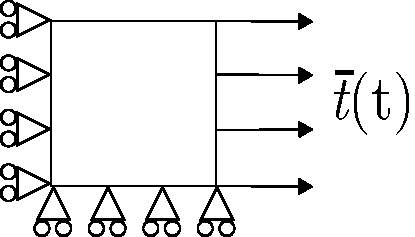
\includegraphics[scale=0.8]{figures/bc_and_ic_example}
  \caption{Plate on movable supports.\label{fig:smm:bc_and_ic}}
\end{figure}


\subsection{Static analysis\label{sect:smm:static}}

The \code{SolidMechanicsModel} class can  handle different analysis methods, the
first one that will be presented is the static case.  In this case, the equation
to solve is,
\begin{equation}\label{eqn:smm:static}
  \mat{K} \vec{u} = \vec{f_{\st{ext}}}
\end{equation}
where  $\mat{K}$ is  the  global stiffness  matrix,  $\vec{u}$ the  displacement
vector  and  $\vec{f_{\st{ext}}}$ the  external  forces  vector  applied to  the
system.


To     solve    such     a    problem     the    static     solver     of    the
\code{SolidMechanicsModel}\index{SolidMechanicsModel}  object is used.   First a
model has to be  created and initialized.  To create the model,  a mesh that can
be read from  a file is needed, as  explained in section \ref{sect:common:mesh}.
Once an instance of a \code{SolidMechanicsModel} is obtained, the easiest way to
initialize it is  to use the \code{initFull}\index{SolidMechanicsModel!initFull}
function by  giving a  material file containing  the material parameters,  and a
type of analysis.

\begin{cpp}
  SolidMechanicsModel model(mesh);
  model.initFull("material.dat", _static);
\end{cpp}


\begin{itemize}
\item \code{model.initFull}  initializes all the  needed vectors to zero.   If a
  material file is given it also  parses it and creates the requested materials.
  The last  parameter of this function  is the type  of solver to use.  Here the
  \code{\_static} solver is used.
\end{itemize}


Once the model is created and  initialized the boundary conditions can be set as
explained   in  section   \ref{sect:smm:boundary}.   Boundary   conditions  will
prescribe   the   external   forces    for   the   free   degrees   of   freedom
$\vec{f_{\st{ext}}}$ and displacements for the others.  To completely define the
system  represented  by equation  (\ref{eqn:smm:static}),  the global  stiffness
matrix            $\mat{K}$             must            be            assembled.
\index{SolidMechanicsModel!assembleStiffnessMatrix}

\begin{cpp}
  model.assembleStiffnessMatrix();
\end{cpp}

In fact, to find the  equilibrium equation (\ref{eqn:smm:static}) is modified in
order to apply a Newton-Raphson convergence algorithm.

\begin{align}\label{eqn:smm:static-newton-raphson}
  \mat{K}^{i+1} \vec{\delta u}^{i+1} &= \vec{r} \\
  &= \vec{f_{\st{ext}}} - \vec{f_{\st{int}}}\\
  &= \vec{f_{\st{ext}}} - \mat{K}^{i} \vec{u}^{i}\\
  \vec{u}^{i+1} &= \vec{u}^{i} + \vec{\delta u}^{i+1}\nonumber
\end{align}
where $\vec{\delta  u}$ is the  increment of displacement  to be added  from one
iteration to the other, and $i$ is the number of the Newton-Raphson iteration.

So  in  a  Newton-Raphson  iteration,  $\mat{K}$ is  updated  according  to  the
displacement computed at  the previous iteration and one  loops until the forces
are balanced, \ie $\vec{r} = 0$.  One can also iterate until the increment of
displacement is zero which also means that the equilibrium is found. This can be
done as follow:
\index{SolidMechanicsModel!updateResidual}
\index{SolidMechanicsModel!solveStatic}

\begin{cpp}
  model.updateResidual();
  model.solveStatic();
\end{cpp}
\begin{itemize}
\item \code{model.updateResidual}  assemble the  internal force and  remove them
  from the external forces.
\item         \code{model.solveStatic}        solve         the        equations
  (\ref{eqn:smm:static-newton-raphson}).   The vector \textbf{increment}  of the
  model   will   contain   the   new   increment  of   displacement,   and   the
  \textbf{displacement} is also updated to the new displacement.
\end{itemize}

For  an   elastic  problem  the  solution   is  directly  found   at  the  first
iteration. But for a non-elastic case, one  needs to iterate as long as the norm
of the residual is not zero (given a specific tolerance).
\begin{cpp}
  Real norm;
  Real tolerance = 1e-3;
  UInt count = 0;
  model.updateResidual();
  while(!model.testConvergenceResidual(tolerance, norm) && (count < 100)) {
    model.solveStatic();
    model.updateResidual();
  };
\end{cpp}

At   the  end   of  the   analysis  the   final  solution   is  stored   in  the
\textbf{displacement} vector.  A  full example of how to  solve a static problem
is  presented  in   the  code  \code{example/manual/implicit\_static.cc}.   This
example is composed of a 2D plate of steel, blocked with rollers on the left and
bottom sides as shown in  Figure \ref{fig:smm:static}.  The nodes from the right
side of the sample are displaced by $0.01\%$ of the length of the plate.

\begin{figure}[!htb]
  \centering
  \includegraphics{figures/implicit_static}
  \caption{Numerical setup\label{fig:smm:static}}
\end{figure}

The     results     of    this     analysis     is     depicted    in     Figure
\ref{fig:smm:implicit:static_solution}.

\begin{figure}[!htb]
  \centering
  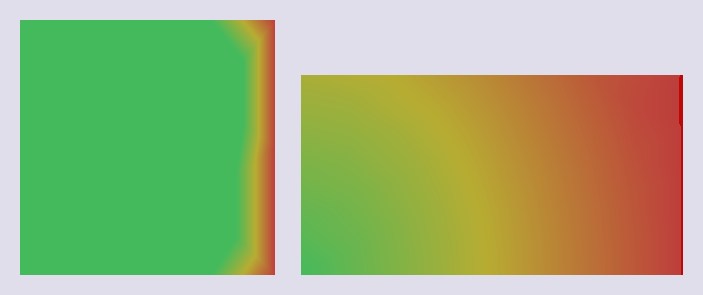
\includegraphics[width=.6\linewidth]{figures/static_analysis}
  \caption{Solution of the static  analysis. Left: the initial condition, right:
    the solution (deformation magnified 50 times)}
  \label{fig:smm:implicit:static_solution}
\end{figure}

\subsection{Dynamic methods} \label{sect:smm:Dynamic_methods}

Different ways  to solve  the equations  of motion are  implemented in  the solid
mechanics model.  The complete equations that should be solved are:
\begin{equation}\label{eqn:equation-motion}
  \mat{M}\vec{\ddot{u}}     +    \mat{C}\vec{\dot{u}}    +     \mat{K}\vec{u}    =
  \vec{f_{\st{ext}}} - \vec{f_{\st{int}}} = \vec{r}
\end{equation}
where $\mat{M}$,  $\mat{C}$ and  $\mat{K}$ are the  mass, damping  and stiffness
matrices respectively.

In  the previous  section,  it has  already  been discussed  how  to solve  this
equation in  the static case where  $\vec{\ddot{u}} = \vec{\dot{u}}  = 0$.  Here
the method  to solve this  equation in the  general case will be  presented.  To
reach  this purpose, a  time discretization  should be  added.  The  most common
discretization method in solid mechanics is the Newmark-$\beta$ method, which is
therefore also the default in \akantu.

For the  Newmark-$\beta$ method, equation  (\ref{eqn:equation-motion}) becomes a
system  of three  equations  (see \cite{curnier92a}  \cite{hughes-83a} for  more
detail):
\begin{align}
  \mat{M}   \vec{\ddot{u}}_{n+1}  +   \mat{C}   \vec{\dot{u}}_{n+1}  +   \mat{K}
  \vec{u}_{n+1} &= \vec{r}_{n+1} \label{eqn:equation-motion-discret} \\
  \vec{u}_{n+1}   &=   \vec{u}_{n}   +   \left(1  -   \alpha\right)   \Delta   t
  \vec{\dot{u}}_{n} + \alpha \Delta  t \vec{\dot{u}}_{n+1} + \left(\frac{1}{2} -
    \alpha\right) \Delta t^2 \vec{\ddot{u}}_{n} \label{eqn:finite-difference-1}\\
  \vec{\dot{u}}_{n+1}  &= \vec{\dot{u}}_{n}  + \left(1  - \beta\right)  \Delta t
  \vec{\ddot{u}}_{n}            +            \beta           \Delta            t
  \vec{\ddot{u}}_{n+1} \label{eqn:finite-difference-2}
\end{align}

In   this   new   equations,   $\vec{\ddot{u}}_{n}$,   $\vec{\dot{u}}_{n}$   and
$\vec{u}_{n}$     are    the     approximations     of    $\vec{\ddot{u}(t_n)}$,
$\vec{\dot{u}(t_n)}$           and           $\vec{u(t_n)}$.            Equation
(\ref{eqn:equation-motion-discret})  is  the  equation  of motion  in  terms  of
approximate  solution  and  the  equations  (\ref{eqn:finite-difference-1})  and
(\ref{eqn:finite-difference-2})  are the  finite difference  formulas describing
the evolution of the approximate solutions.  The $\alpha$ and $\beta$ parameters
determine the stability and the  accuracy of the algorithm. Classical values for
$\alpha$ and $\beta$ are usually $\beta = 1/2$ for no numerical damping and $0 <
\alpha < 1/2$.

\begin{center}
  \begin{tabular}{cll}
    \toprule
    $\alpha$ & Method ($\beta = 1/2$) & Type\\
    \midrule
    $0$ & central difference & explicit\\
    $1/6$ & Fox-Goodwin (royal road) &implicit\\
    $1/3$ & Linear acceleration &implicit\\
    $1/2$ & Average acceleration (trapezoidal rule)& implicit\\
    \bottomrule
  \end{tabular}
\end{center}

To     be      able     to      solve     this     system      of     equations,
(\ref{eqn:equation-motion-discret})-(\ref{eqn:finite-difference-2})   should  be
split in a predictor-corrector system of  equations.  Moreover, in the case of a
non-linear equation as  for the static case, an iterative  algorithm such as the
Newton-Raphson method is applied.  According  to these conditions, the system of
equations can be written as:

\noindent\textit{Predictor:}
\begin{align}
  \vec{u}_{n+1}^{0} &=  \vec{u}_{n} +  \Delta t \vec{\dot{u}}_{n}  + \frac{\Delta
    t^2}{2} \vec{\ddot{u}}_{n} \\
  \vec{\dot{u}}_{n+1}^{0}  &= \vec{\dot{u}}_{n} +  \Delta t \vec{\ddot{u}}_{n} \\
  \vec{\ddot{u}}_{n+1}^{0} &= \vec{\ddot{u}}_{n}
\end{align}

\noindent\textit{Solve:}
\begin{align}
  \left(c \mat{M} + d \mat{C}  + e \mat{K}_{n+1}^i\right) \vec{w} = \vec{f_{\st{ext}}}_{n+1} -
  \vec{f_{\st{int}}}_{n+1}^i    -   \mat{C}    \vec{\dot{u}}_{n+1}^i    -   \mat{M}
  \vec{\ddot{u}}_{n+1}^i
\end{align}

\noindent\textit{Corrector:}
\begin{align}
  \vec{\ddot{u}}_{n+1}^{i+1} &= \vec{\ddot{u}}_{n+1}^{i} + c \vec{w} \\
  \vec{\dot{u}}_{n+1}^{i+1} &= \vec{\dot{u}}_{n+1}^{i} + d \vec{w} \\
  \vec{u}_{n+1}^{i+1} &= \vec{u}_{n+1}^{i} + e \vec{w}
\end{align}

where  $i$ is  the Newton-Raphson  iteration counter  and $c$,  $d$ and  $e$ are
parameters depending on the method used to solve the equations

\begin{center}
  \begin{tabular}{lcccc}
    \toprule
    & $\vec{w}$ & $e$ & $d$ & $c$\\
    \midrule
    in  acceleration  &$ \vec{\delta  \ddot{u}}$  &  $\alpha  \beta \Delta  t^2$
    &$\beta \Delta t$ &$1$\\
    in velocity  & $ \vec{\delta \dot{u}}$&  $\frac{1}{\beta} \Delta t$  & $1$ &
    $\alpha \Delta t$\\
    in displacement  &$\vec{\delta u}$  & $ 1$  & $\frac{1}{\alpha} \Delta  t$ &
    $\frac{1}{\alpha \beta} \Delta t^2$\\
    \bottomrule
  \end{tabular}
\end{center}

\note{If you want to use the implicit solver \akantu should be compiled at least
  with one sparse matrix solver such as Mumps\cite{mumps}.}


\subsubsection{Implicit time integration}
To  solve  a  problem with  an  implicit  time  integration scheme,  first  a
\code{SolidMechanicsModel} object  should be created and  initialized.  Then the
initial and  boundary conditions have to  be set.  Everything is  similar to the
example  in static case  (section \ref{sect:smm:static}),  however in  this case
during  the initialization of  the model,  the implicit  dynamic case  should be
selected.

\begin{cpp}
  SolidMechanicsModel model(mesh);
  model.initFull("material.dat", _implicit_dynamic);
  /* Boundary conditions see section %\ref{sect:smm:boundary}% */
\end{cpp}

Then, the  stiffness matrix  $\mat{K}$ and the  mass matrix $\mat{M}$  should be
assembled.  Since  the material is  elastic in this  case $\mat{C}$ is  equal to
zero.
\index{SolidMechanicsModel!assembleStiffnessMatrix}
\index{SolidMechanicsModel!assembleMass}
\begin{cpp}
  model.assembleStiffnessMatrix();
  model.assembleMass();
\end{cpp}

Since  a dynamic  simulation is  conducted, a  time step  $\Delta t$  has  to be
specified. In the case of  implicit simulations, \akantu implements a trapezoidal
rule by  default.  That  is to say  $\alpha =  1/2$ and $\beta  = 1/2$  which is
unconditionally  stable. Therefore  the value  of the  time step  can  be chosen
arbitrarily.  \index{SolidMechanicsModel!setTimeStep}
\begin{cpp}
  model.setTimeStep(time_step);
\end{cpp}

At this point everything is set up to perform the time iterations. The time loop
should  contain the  predictor, the  solving and  the corrector  steps  with the
Newton-Raphson convergence algorithm even if the material is linear.  By default
the        equations       are       solved        \emph{in       displacement}.
\index{SolidMechanicsModel!implicitPred}
\index{SolidMechanicsModel!implicitCorr}
\index{SolidMechanicsModel!updateResidual}
\index{SolidMechanicsModel!solveDynamic}
\begin{cpp}
  for (Real time = 0; time < simulation_time; time += time_step) {
    model.implicitPred();

    UInt count = 0;
    /// Newton-Raphson convergence loop
    do {
      model.updateResidual();
      model.solveDynamic();

      model.implicitCorr();
      ++count;
    } while(!model.testConvergenceIncrement(1e-12, error) && count < 100);
  }
\end{cpp}

\note{In  case of  an  elastic material  $\mat{K}$  is constant,  but for  other
  materials $\mat{K}$ has to be re-assembled at each iteration.}

\note{For the convergence loop  it is a good usage to put  also a limit in terms
  of the  number of iterations  to avoid  an infinite loop  in case of  an error
  criterion too hard to reach.}

An    example    of    implicit    dynamic   analysis    is    presented    here
\code{example/manual/implicit\_dynamic.cc}.  This example  consists of a 2D beam
of $\unit{10}{\meter}\,\times\,\unit{1}{\meter}$ blocked on one side and is on a
roller on the other side.  A constant force of \unit{5}{\kilo\newton} is applied
in the middle of  this beam.  Figure \ref{fig:smm:implicit:dynamic} presents the
geometry of this case. The material used is a linear fictitious elastic material
with  a density  of  \unit{1000}{\kilogrampercubicmetre}, a  Young's Modulus  of
\unit{120}{\mega\pascal} and Poisson's ratio  of $0.3$. These values were chosen
to simplify the analytical solution.

An approximation  of the  dynamic response of  the middle  point of the  beam is
given by:
\begin{equation}\label{eqn:smm:implicit}
  u\left(\frac{L}{2}, t\right) = \frac{1}{\pi^4} \left(1 - cos\left(\pi^2 t\right) +
    \frac{1}{81}\left(1 - cos\left(3^2 \pi^2 t\right)\right) +
    \frac{1}{625}\left(1 - cos\left(5^2 \pi^2 t\right)\right)\right)
\end{equation}

\begin{figure}[!htb]
  \centering
  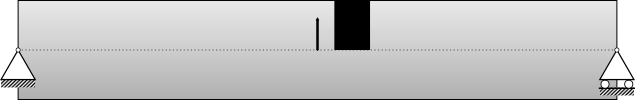
\includegraphics[scale=.6]{figures/implicit_dynamic}
  \caption{Numerical setup}
  \label{fig:smm:implicit:dynamic}
\end{figure}

Figure \ref{fig:smm:implicit:dynamic_solution}  presents the deformed  beam at 3
different times of the simulation, time steps 0, 1000 and 2000.

\begin{figure}[!htb]
  \centering
  \setlength{\unitlength}{0.1\textwidth}
  \begin{tikzpicture}
    \node[above right] (img) at (0,0)
    {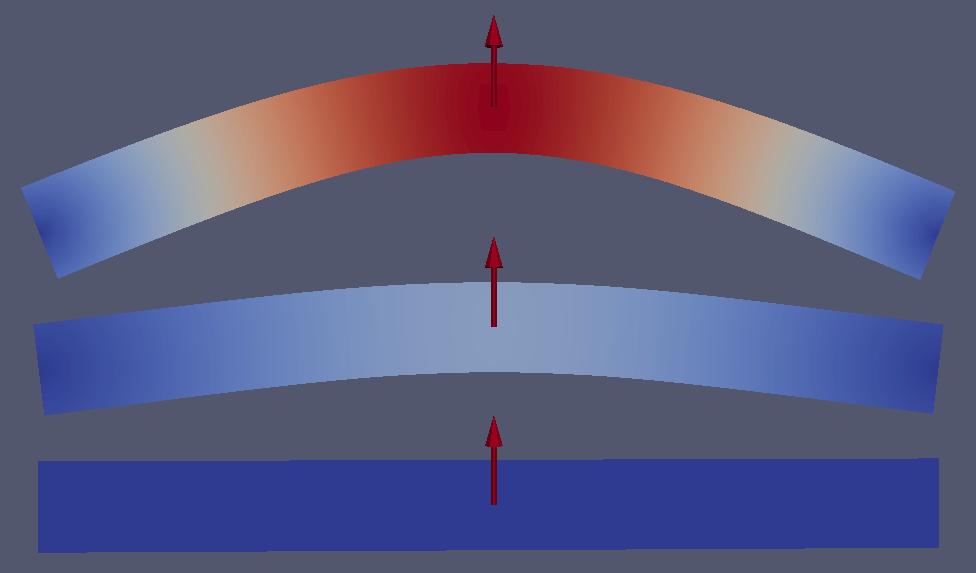
\includegraphics[width=.6\linewidth]{figures/dynamic_analysis}};
    \node[left] at (0pt,20pt) {$0$};
    \node[left] at (0pt,60pt) {$1000$};
    \node[left] at (0pt,100pt) {$2000$};
  \end{tikzpicture}

  \caption{Deformed beam at 3 different time (displacement are
    magnified by a factor 10).}
  \label{fig:smm:implicit:dynamic_solution}
\end{figure}

\subsubsection{Explicit dynamic}

The explicit  dynamic time  integration scheme is  based on  the Newmark-$\beta$
scheme            with            $\alpha=0$           (see            equations
\ref{eqn:equation-motion-discret}-\ref{eqn:finite-difference-2}).   In  \akantu,
$\beta$ is defined as $\beta=1/2$, see section \ref{sect:smm:Dynamic_methods}.

The  initialization of  the simulation  is similar  to the  static  and implicit
dynamic  version.   The model  is  created  from the  \code{SolidMechanicsModel}
class.   In the  initialization, the  use of  the explicit  scheme  should be
defined with the \code{\_explicit\_dynamic} keyword.

\begin{cpp}
  SolidMechanicsModel model(mesh);
  model.initFull("material.dat", _explicit_dynamic);
\end{cpp}
\index{SolidMechanicsModel!initFull}

\note{Writing \code{model.initFull("material.dat");}  is equivalent to  use the
  \code{\_explicit\_dynamic} keyword, as this is the default case.}

The implemented explicit  time integration scheme in \akantu  uses a lumped mass
matrix $\mat{M}$ (reducing the computational  cost). This matrix is assembled by
distributing the mass of each element onto its nodes. The resulting $\mat{M}$ is
therefore a diagonal matrix stored in the \textbf{mass} vector of the model.


\begin{cpp}
  model.assembleMassLumped();
\end{cpp}
\index{SolidMechanicsModel!assembleMassLumped}

The explicit integration scheme is conditionally stable. The time step has to be
smaller than the stable time step which is obtained in \akantu as follows:

\begin{cpp}
  time_step = model.getStableTimeStep();
\end{cpp}
\index{SolidMechanicsModel!StableTimeStep}

The stable time step is defined as:
\begin{equation}\label{eqn:smm:explicit:stabletime}
  \Delta t_{\st{crit}} = \Delta x \sqrt{\frac{\rho}{2 \mu +\lambda}}
\end{equation}
where $\Delta  x$ is a  characteristic length (\eg  the inradius in the  case of
linear triangle  element), $\mu$ and $\lambda$  are the first  and second Lame's
coefficients and $\rho$ is the density.  The stable time step corresponds to the
time the fastest wave (the  compressive wave) needs to travel the characteristic
length of the mesh.   However, note that if the time step  of the computation is
equal to the stable time step, the simulation remains unstable. Therefore, is it
necessary to impose a  time step that is smaller than the  stable time step, for
instance, by  multiplying the stable time  step by a safety  factor smaller than
one.

\begin{cpp}
  const Real safety_time_factor = 0.1;
  Real applied_time_step = time_step * safety_time_factor;
  model.setTimeStep(applied_time_step);
\end{cpp}
\index{SolidMechanicsModel!setTimeStep}

The initial displacement  and velocity fields are, by default,  equal to zero if
not given specifically by the user (see \ref{sect:smm:initial_condition}).

The loop  allows, for each time  step, to update the  displacement, velocity and
acceleration  fields  which are  given  by  the  Newmark$-\beta$ equations  with
$\beta=1/2$ and $\alpha=0$.

\begin{cpp}
  for (UInt s = 1; (s-1)*applied_time_step < total_time; ++s) {
    model.explicitPred();
    model.updateResidual();
    model.updateAcceleration();
    model.explicitCorr();
  }
\end{cpp}
\index{SolidMechanicsModel!explicitPred}
\index{SolidMechanicsModel!explicitCorr}
\index{SolidMechanicsModel!updateResidual}
\index{SolidMechanicsModel!updateAcceleration}

In the code shown above, the explicit loop contains four steps:
\begin{itemize}
\item \code{model.explicitPred()}  allows to  compute the displacement  field at
  $t+1$   and   a  part   of   the  velocity   field   at   $t+1$,  denoted   by
  $\vec{\dot{u}_{n+1/2}}$,    which    will     be    used    later    in    the
  \code{model.explicitCorr()}. The solved equations are:

  \begin{align}
    \vec{u}_{n+1}  &= \vec{u}_{n}  + \Delta  t \vec{\dot{u}}_{n}  + \frac{\Delta
      t^2}{2} \vec{\ddot{u}}_{n}\\
    \vec{\dot{u}_{n+1/2}}  &= \vec{\dot{u}}_{n} +  \Delta t  \vec{\ddot{u}}_{n}
    \label{eqn:smm:explicit:onehalfvelocity}
  \end{align}

\item \code{model.updateResidual()}  and \code{model.updateAcceleration()} allow
  to  solve  the  equation   which  gives  the  acceleration  increment  $\delta
  \vec{\ddot{u}}$:

  \begin{equation}
    \left(\mat{M}  +  \frac{1}{2}  \Delta  t \mat{C}\right)  \delta  \vec{\ddot{u}}  =
    \vec{f_{\st{ext}}} -  \vec{f}_{\st{int}n+1} - \mat{C}  \vec{\dot{u}}_{n} -
    \mat{M} \vec{\ddot{u}}_{n}
  \end{equation}

  \note{The  internal   force  $\vec{f}_{\st{int}n+1}$  is   computed  from  the
    displacement $\vec{u}_{n+1}$ based on the constitutive law.}

\item \code{model.explicitCorr()} computes  the velocity and acceleration fields
  at $t+1$:

  \begin{align}
    \vec{\dot{u}}_{n+1}  &= \vec{\dot{u}}_{n+1/2} + \frac{\Delta t}{2} \delta \vec{\ddot{u}} \\
    \vec{\ddot{u}}_{n+1}  &= \vec{\ddot{u}}_{n} +  \delta \vec{\ddot{u}}
  \end{align}
\end{itemize}

The use  of the explicit  time integration scheme  is illustrated by  an example
(see  \code{example/manual/explicit\_dynamic.cc}).    This  example  models  the
propagation of  a wave in a  steel beam. The beam  is blocked on one  side and a
displacement   is   applied   on   the   other  side,   as   shown   in   figure
\ref{fig:smm:explicit}.

\begin{figure}[!htb]
  \centering
  \includegraphics[scale=.6]{figures/explicit_dynamic}
  \caption{Numerical setup \label{fig:smm:explicit}}
\end{figure}

The length  and height of  the beam are \unit{10}{\metre}  and \unit{1}{\metre},
respectively.   The  material  is  linear  elastic,  homogeneous  and  isotropic
(density:       \unit{7800}{\kilogrampercubicmetre},       Young's      modulus:
\unit{210}{\giga\pascal} and Poisson's  ratio: $0.3$).  The imposed displacement
is equal to  $\Delta u = \unit{0.05}{\metre}$. The  potential, kinetic and
total  energies are  computed.  The  time factor  is equal  to $0.1$.  The total
simulated time is \unit{0.01}{\second}.

\subsection{Constitutive laws \label{sect:smm:CL}}
In order to compute an element's response to deformation, one needs to use an appropriate constitutive relationship for every element in the mesh. The constitutive law enables to compute the element's stresses from the element's strains. In the finite element discretization, the constitutive formulation is applied to every quadrature point of each element.

The chosen materials for the virtual simulation have to be specified in the mesh file or as an alternative they can be assigned using the \code{element\_material} vector.
For every material assigned to the problem one has to specify the material characteristics (constitutive behavior and material properties) in a text file (\eg material.dat) as follows:
\begin{cpp}
  material %\emph{constitutive\_law}% [
  name = %\emph{XXX}%
  rho = %\emph{XXX}%
  % $\vdots$%
  ]

\end{cpp}
\index{Constitutive_laws}
where \emph{constitutive\_law} is the adopted constitutive law, followed by the material properties listed one by line in the bracket (\eg \code{name} and density \code{rho}). The file needs to be loaded in \akantu using the \code{readMaterials} method
\begin{cpp}
  model.readMaterials("material.dat");
\end{cpp}
or in alternative the \code{initFull} method.
\begin{cpp}
  model.initFull("material.dat");
\end{cpp}
The following subsections describe the constitutive models implemented in \akantu.

\subsubsection{Elastic}
The elastic law is a commonly used constitutive relationship that can be used for a wide range of engineering materials (\eg metals, concrete, rock, wood, glass, rubber, etc.) provided that the strains remain small (\ie small deformation and stress lower than yield strength). The linear elastic behavior is described by Hooke's law, which states that the stress is linearly proportional to the applied strain (material behaves like an ideal spring), as illustrated in Figure~\ref{fig:smm:cl:elastic}.
\begin{figure}[!htb]
  \begin{center}

    \subfloat[]{
      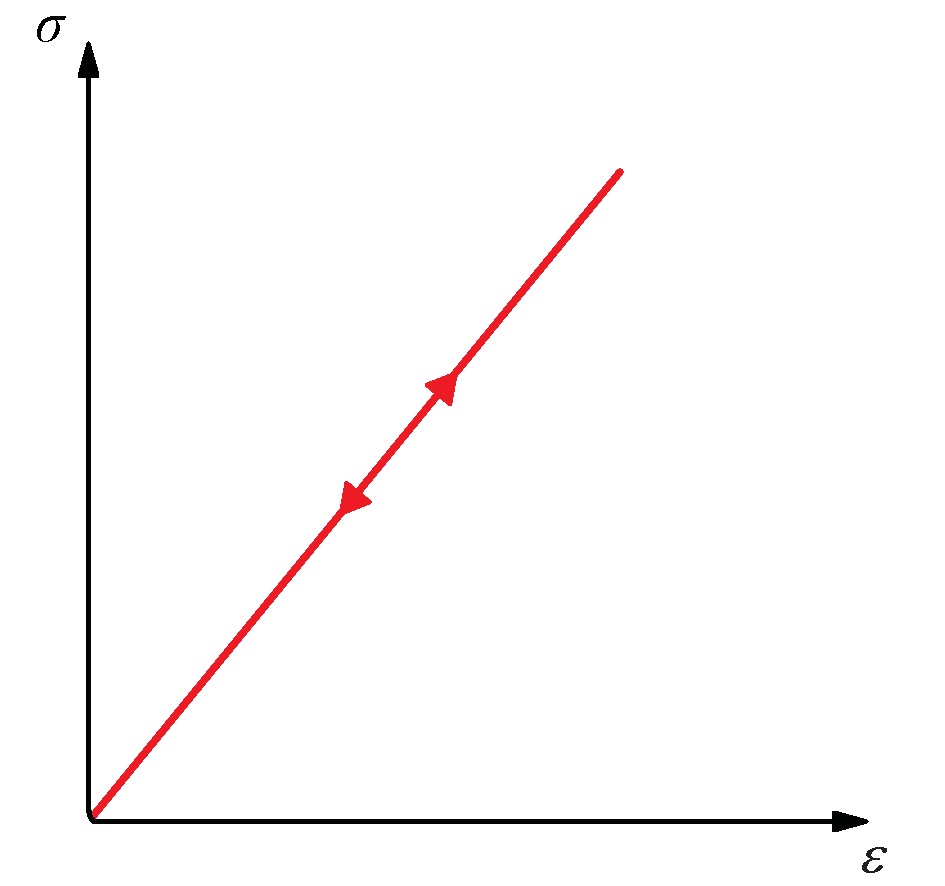
\includegraphics[width=0.4\textwidth,keepaspectratio=true]{figures/stress_strain_el.pdf}
      \label{fig:smm:cl:elastic:stress_strain}
    }
    \hspace{0.05\textwidth}
    \subfloat[]{
      \raisebox{0.125\textwidth}{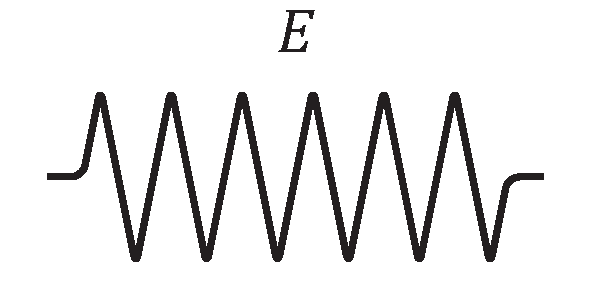
\includegraphics[width=0.25\textwidth,keepaspectratio=true]{figures/hooke_law.pdf}}
      \label{fig:smm:cl:elastic:hooke}
    }
    \caption{(a) Stress-strain curve for elastic material and (b) schematic representation of Hooke's law, denoted as a spring.}
    \label{fig:smm:cl:elastic}
  \end{center}
\end{figure}
The equation that relates the strains to the displacements is:
% First the strain is computed (at every gauss point) from the displacements as follows:
\begin{equation}\label{eqn:smm:strain_inf}
  \mat{\epsilon} = \frac{1}{2} \left[ \mat{F}-\mat{I}+(\mat{F}-\mat{I})^T \right]
\end{equation}
where $\mat{\epsilon}$ represents the infinitesimal strain tensor, $\mat{F} = \nabla_{\vec{X}}\vec{x}$ the deformation gradient tensor and $\mat{I}$ the identity matrix. The constitutive equation for isotropic homogeneous media can be expressed as:
\begin{equation}\label{eqn:smm:constitutive_elastic}
  \mat{\sigma } =\lambda\mathrm{tr}(\mat{\epsilon})\mat{I}+2 \mu \mat{\epsilon}
\end{equation}
where $\mat{\sigma}$ is the Cauchy stress tensor ($\lambda$ and $\mu$ are the the first  and second Lame's coefficients). Besides the name and density, one has to specify the following properties in the material file: \code{E} (Young's modulus), \code{nu} (Poisson's ratio) and (for 2D) \code{Plain\_Stress} (if set to zero or not specified plane strain conditions are assumed for a plain analysis, otherwise plane stress conditions are applied).

\subsubsection{Caughey}
** Not in release **
The model is a particular case of the Rayleigh damping model, with damping being proportional only to the stiffness matrix. Substitute with complete Rayleigh damping model for release?

\subsubsection{Neo-Hookean}
The Neo-Hookean constitutive law is a hyperelastic material formulation, which results from an extension of the linear elastic relationship (Hooke's Law) for large deformation. Thus, the model predicts nonlinear stress-strain behavior for bodies undergoing large deformations.

\begin{figure}[!htb]
  \begin{center}
    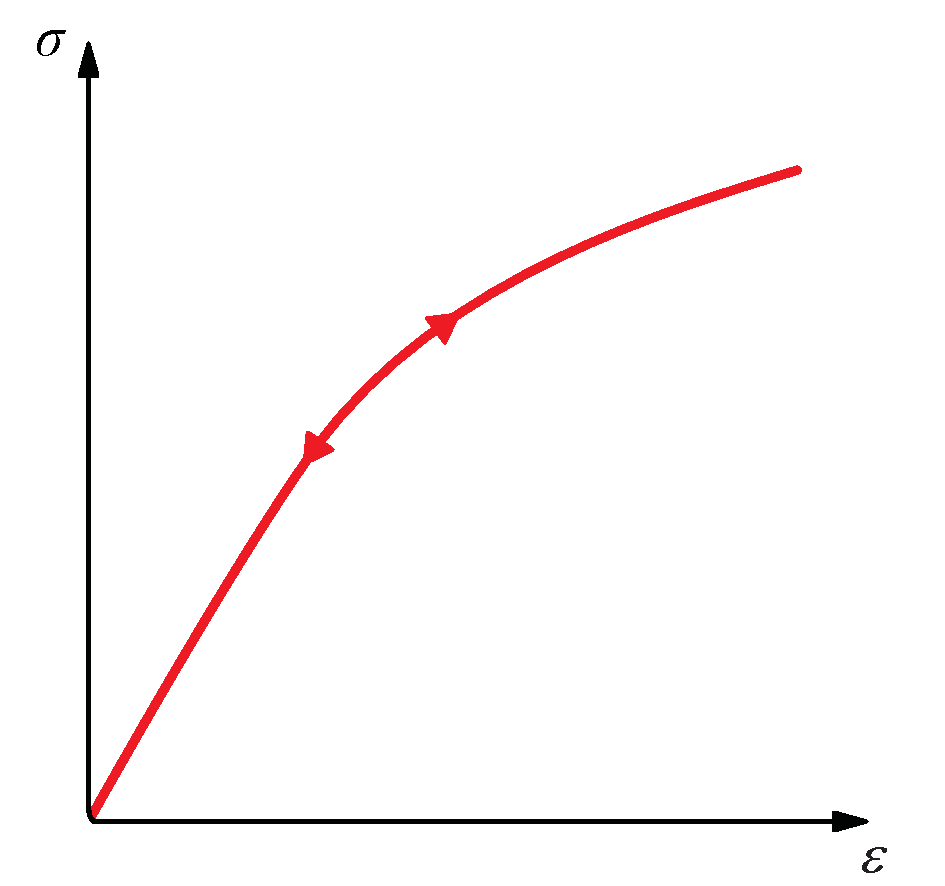
\includegraphics[width=0.4\textwidth,keepaspectratio=true]{figures/stress_strain_neo.pdf}
    \caption{Neo-hookean Stress-strain curve.}
    \label{fig:smm:cl:neo_hookean}
  \end{center}
\end{figure}

As illustrated in Figure~\ref{fig:smm:cl:neo_hookean}, the behavior is initially linear but at a certain point it will start to converge to a plateau.
This constitutive relationship has been proposed by Ronald Rivlin and is suitable to simulate rubber-like (\eg polymers) material behavior. The constitutive equation is 
\begin{equation}
  \mat{\sigma } = -p \mat{I} + \mu \mat{B}
\end{equation}
where $p$ is the pressure and $\mat{B}$ is the Finger deformation tensor ($\mat{B}=\mat{F}^{-1}\mat{F}^{-T}$) and $\mat{F}$, as before, the deformation gradient tensor.
The parameters to indicate in the material file are the same as those for the elastic case: \code{E} (Young's modulus), \code{nu} (Poisson's ratio) and \code{Plain\_Stress} (if set to zero plane strain, else plane stress).

\subsubsection{Visco-elastic (IMPLEMENTATION TO VERIFY!!)}

% Standard Solid rheological model, see [] J.C. Simo, T.J.R. Hughes, "Computational Inelasticity", Springer (1998), see Sections 10.2 and 10.3
Visco-elasticity is characterized by time dependent strain behavior. Moreover, when such a material undergoes a deformation it dissipates some energy. This dissipation results in a hysteresis loop in the stress-strain curve at every loading cycle (see Figure~\ref{fig:smm:cl:visco-elastic:hyst}). In principle, it can be applied to many materials, since all materials exhibit a visco-elastic behavior if subjected to particular conditions (such as high temperatures).
\begin{figure}[!htb]
  \begin{center}

    \subfloat[]{
      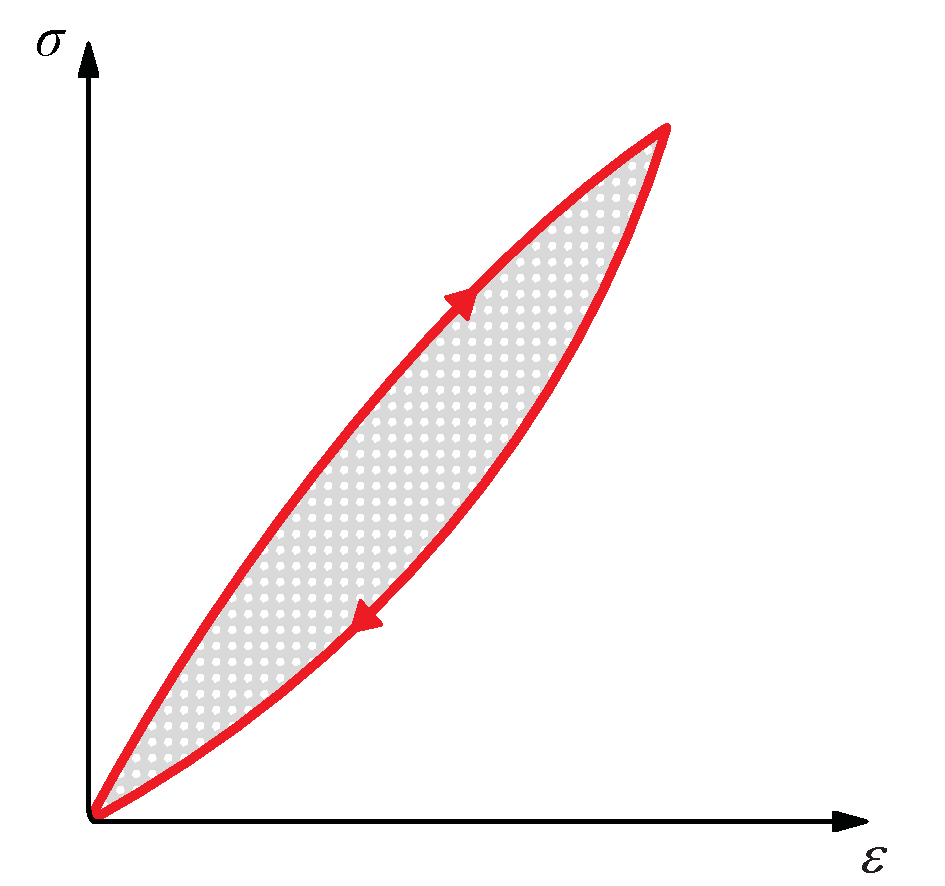
\includegraphics[width=0.4\textwidth,keepaspectratio=true]{figures/stress_strain_visco.pdf}
      \label{fig:smm:cl:visco-elastic:hyst}
    }
    \hspace{0.05\textwidth}
    \subfloat[]{
      \raisebox{0.025\textwidth}{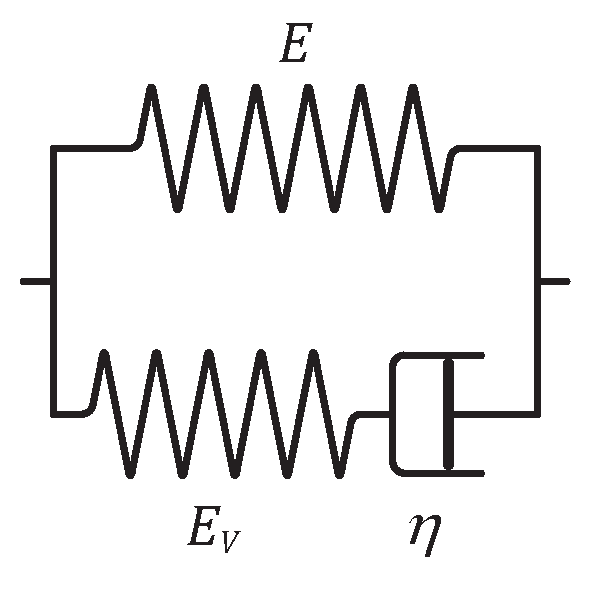
\includegraphics[width=0.3\textwidth,keepaspectratio=true]{figures/visco_elastic_law.pdf}}
      \label{fig:smm:cl:visco-elastic:model}
    }
    \caption{(a) Characteristic stress-strain behavior of a visco-elastic material with hysteresis loop and (b) schematic representation of the standard rheological linear solid visco-elastic model.}
    \label{fig:smm:cl:visco-elastic}
  \end{center}
\end{figure}
The standard rheological linear solid model (see Sections 10.2 and 10.3 of~\cite{simo92}) has been implemented in \akantu. This model results from the combination of a spring mounted in parallel with a spring and a dashpot connected in series, as illustrated in Figure~\ref{fig:smm:cl:visco-elastic:model}. The advantage of this model is that it allows to account for creep and stress relaxation. The equation that relates the stress to the strain is (in 1D):
\begin{equation}
  \frac{d\epsilon(t)}{dt} = \left ( E + E_V \right ) ^ {-1} \cdot \left [ \frac{d\sigma(t)}{dt} + \frac{E_V}{\eta}\sigma(t) - \frac{EE_V}{\eta}\epsilon(t) \right ]
\end{equation}
where $\eta$ is the viscosity. The equilibrium condition is unique and is attained in the limit, as $t \to \infty $. At this stage, the response is elastic and depends on the Young's modulus $E$.
The parameters requested in the material file are the following: \code{rho} (density), \code{E} (Young's modulus), \code{nu} (Poisson's ratio), \code{Plane\_Stress} (if set to zero plane strain, otherwise plane stress), \code{eta} (dashpot viscosity) and \code{Ev} (stiffness of the viscous element).

\subsubsection{Damage Marigo}
\subsubsection{Damage Mazars}

\subsection{Adding a new constitutive law}


There are  several existing constitutive laws in  \akantu as described
in the  previous Section \ref{sect:smm:CL};  it is also  possible to
add a new constitutive relationship which indicates a new material to the
current ones. To define a new plugin material, two files (\code {material\_XXX.cc} and
\code{material\_XXX.hh}) should be provided where \code{XXX} is the name of
the new material. In the \code{material\_XXX.hh} the interface of the custom material
should be given and in the \code{material\_XXX.cc} the implementation of
the functions should be presented.  The new law has to inherit from
the material class or any other existing \code{Material} class and the
following functions have to be redefined for the new constitutive law.


\begin{cpp}
  void initMaterial();

  bool setParam(const string & key, const string & value,
  const ID & id);

  void computeStress(ElementType el_type, GhostType ghost_type = _not_ghost);

  void computeTangentStiffness(const ElementType & el_type,
  Vector<Real> & tangent_matrix,
  GhostType ghost_type = _not_ghost);

  Real getStableTimeStep(Real h, const Element & element);

  void printself(ostream & stream, int indent = 0) const;
\end{cpp}


For each material, the minimum required parameters has to be defined in
a material file.  For existing materials, as mentioned in section
\ref{sect:smm:CL}, one can use a \code{readMaterials}
or \code{initFull} function for reading a material file. However, for reading the parameters of
the  \textbf{plugin} material  law  \code{readCustomMaterial} function
should be used. Some of  these parameters can  be initialized  in the
constructor. Moreover, some internal values can be considered
for  each  quadrature  point,  which   can  be  also  initialized  in  the
constructor of the new law with the
function \code{initInternalVector}. These internal
members have a \code{ByElementTypeReal} type which means they are
real values that are considered for each of the quadrature points of the elements.



Finally,    the    class   members    should    be    declared   in    the
\code{material\_XXX.hh} file. In the following, each required function is described.


\begin{itemize}

\item \code{setParam}  This function  is called for each  line of the material  file. As described before, the lines of
  this file is as following:
  \begin {cpp}
    key = value;
  \end{cpp}
  If the key of the parameter is known in
  this  function  it  will  be   stored  otherwise  it  will  call  the
  \code{setParam} of the parent class to set it.
  Therefore, the parameters which are specially made for the new material
  can be stored as following.

  \begin{cpp}
    stringstream sstr(value);
    if(key == "E") { sstr >> E; }
    else if(key == "nu") { sstr >> nu; }
    else if(key == "Plane_Stress") { sstr >> plane_stress; }
    else { return Material::setParam(key, value, id); }
  \end{cpp}

\item \code{initMaterial} This function is called after the material file is fully read and the
  elements  corresponding  to  each  material are  assigned.  In  this
  function, some of the constant parameters which
  are frequently used are calculated. For example, for the 
  elastic material the Lame's constants  can be considered as these kinds
  of parameters.  Moreover, the  internal members can  be resized  with
  \code{resizeInternalVector} function to the number of the quadrature
  points handled by the material.

\item \code{computeStress}  In this function the stresses are computed based on the constitutive
  law knowing the  strains for the quadrature points.  For example, for
  the  elastic  material the  stresses  are  calculated  based on  the
  following formula: 

 \begin{equation}\label{eqn:smm:constitutive_elastic}
    \mat{\sigma } =\lambda\mathrm{tr}(\mat{\epsilon})\mat{I}+2 \mu \mat{\epsilon}
  \end{equation}

Therefore, this
  function contains  a loop on  all quadrature points assigned  to the
  material                          using                          the
  \code{MATERIAL\_STRESS\_QUADRATURE\_POINT\_LOOP\_BEGIN;}               and
  \code{MATERIAL\_STRESS\_QUADRATURE\_POINT\_LOOP\_END;}  macros.  For
  example in  the following  the components of  the strain  matrix are
  stored in a temporary matrix (F).

  \begin{cpp}
    MATERIAL_STRESS_QUADRATURE_POINT_LOOP_BEGIN;
    
// stress_val <- f(strain_val)
   
    MATERIAL_STRESS_QUADRATURE_POINT_LOOP_END;
  \end{cpp} 

 \note{ This  function can be split  in two functions.  In other words,
   the calculation of the stress for a quadrature point can be done in
   an inline function which is stored in a file such as \code{material\_XXX\_inline.cc}.}
  
\note{  The strain  vector  in  \akantu contains  the  values of  the
  $\nabla \vec{u}$.}


\item \code{computeTangentStiffness}  This function is called when  the tangent to the stress-strain curve
  is desired (see Fig \ref {fig:smm:AL:K}).  For example, it is called in the implicit solver when
  the stiffness matrix for the regular elements is assembled based on the following formula:

  \begin{equation} \label{eqn:smm:constitutive_elasc}
    \mat{K } =\int{\mat{B^T}\mat{D(\epsilon)}\mat{B}}
  \end{equation}

Therefore, in this function the \code{tangent} matrix (\mat{D}) is computed for a given strain. 

\note{ The \code{tangent}  matrix is a $4^{th}$ order  tensor which is
  stored as a matrix in the Voigt notation.}
  
  \begin{figure}[!htb]
    \begin{center}
      \includegraphics[width=0.4\textwidth,keepaspectratio=true]{figures/tangent.pdf}
      \caption{Tangent to the stress-strain curve.}
      \label{fig:smm:AL:K}
    \end{center}
  \end{figure}


\item \code{getStableTimeStep} For the dynamic methods the stable
  time     step    should     be    calculated     based     on    the
  equation \ref{eqn:smm:explicit:stabletime}.  This function depends
  on longitudinal wave speed which changes for different materials and strains. Therefore, the  value of
  this  velocity should  be  defined  in this  function  for each  new
  material. 

  \note  {In case  of need,  the calculation  of the  longitudinal and
    shear wave speeds can be done in separate functions (\code{getPushWaveSpeed} and
  \code{getShearWaveSpeed}).  Therefore,  the  first  function  can  be
  called for calculation of the stable time step.} 

\item \code{printself} The final function which should be redefined is
  a function to print out
  the information of the material law. The interface of this function
  is similar to the one for existing laws. This function will write on
  the output the required material information. 
\end{itemize}

  A full example for adding a new damage law can be
  found in \code{example/manual/new\_material}. 


\subsection{Contact\todo{Alejendro, David, Vlad}}

\subsection{Cohesive laws\todo{Marco}}


\section{Structural Mechanics model\todo{Till}}

\section{Heat Transfer model\todo{Guillaume}}

% \subsection{Contact Neighbor Structure}

% The contact neighbor  structure is an interface which is  ment to be heritated
% from in order  to implement different type of  contact neighbor structures. It
% has the following protected attributes:
% \begin{itemize}
% \item id
% \item contact search
% \item master surface
% \item neighbor list
% \item type
% \end{itemize}
% The \emph{id} and the \emph{type}  are characteristics of the contact neighcor
% structure object which  define its id and its  type. The \emph{contact search}
% attribute  is  the associated  contact  search  object  to the  given  contact
% neighbor structure  object. The \emph{master  surface} attribute is the  id of
% the  associated master  surface for  which the  neighbor structure  has  to be
% built. Finally, the neighbor list  is the constructed neighbor structure which
% defines the  impactor nodes  that are  in the neighborhood  of either  a given
% master  node or  a given  master  surface element,  depending on  the type  of
% contact neighbor structure.

% The contact neighbor structure provides the accessor \emph{getNeighborList} to
% the constructed  neighbor list and forces  the heritated classes  to provide a
% public \emph{initNeighborStructure}  function, which initializes  the neighbor
% structure,  as well  as a  public  \emph{update} function,  which updates  the
% neighbor structure.

% \subsubsection{Regular Grid Neighbor Structure}

% The regular  grid neighbor structure builds  a regular grid  around the master
% surface and  uses it in  order to construct  the neighbor list.  This neighbor
% structure can construct both types of neighbor list, the


% \subsection{Implementation of a new solid mechanics problem}

% Let us imagine you want to implement a new material called
% "toto" in akantu. The have to complete the following steps (in
% any order) :
% \begin{enumerate}
% \item
%   Declare a new material in the file
%   \textit{Akantu/model/solid\_mechanics/solid\_mechanics\_model\_material.cc}.
%   You have to had this line after the list of possible cases
% \begin{verbatim}else if(mat\_type == "toto") material =
% parser.readMaterialObject<MaterialToto>(*this,mat_id);
% \end{verbatim}


% \item
%   Include the new material in \textit{Akantu/model/solid\_mechanics/material.hh} \\
%   add the line :
% \begin{verbatim}
% #include "materials/material\_toto.hh"
% \end{verbatim}

% \item
%   For compilation include the new file to compile in
%   \textit{Akantu/CMakelist.txt} by adding
% \begin{verbatim}
% model/solid_mechanics/materials/material_toto.cc
% \end{verbatim}
% \item
%   In \textit{Akantu/model/solid\_mechanics/materials}, create (or copy from
%   an allready existing material) the three following files :\\
%   - material\_toto.cc\\
%   - material\_toto.hh\\
%   - material\_toto\_inline\_impl.cc

% \item
%   Modify the files !

% \end{enumerate}
\printindex

\bibliography{biblio}


\end{document}
